%! Licence = CC BY-NC-SA 4.0

%! Author = mariuszindel
%! Date = 06. Jul 2021
%! Project = DS1-Summary

\section{Deployment}

\subsection{Kubernetes}
\subsubsection{Properties}
\begin{itemize}
    \item Configuration is declarative – declare state with YAML/JSON 
    \item Abstraction layer for distributed system
    \item Immutable containers (Don’t store state in a container)
    \item Master / worker architecture
\end{itemize}
\begin{center}
    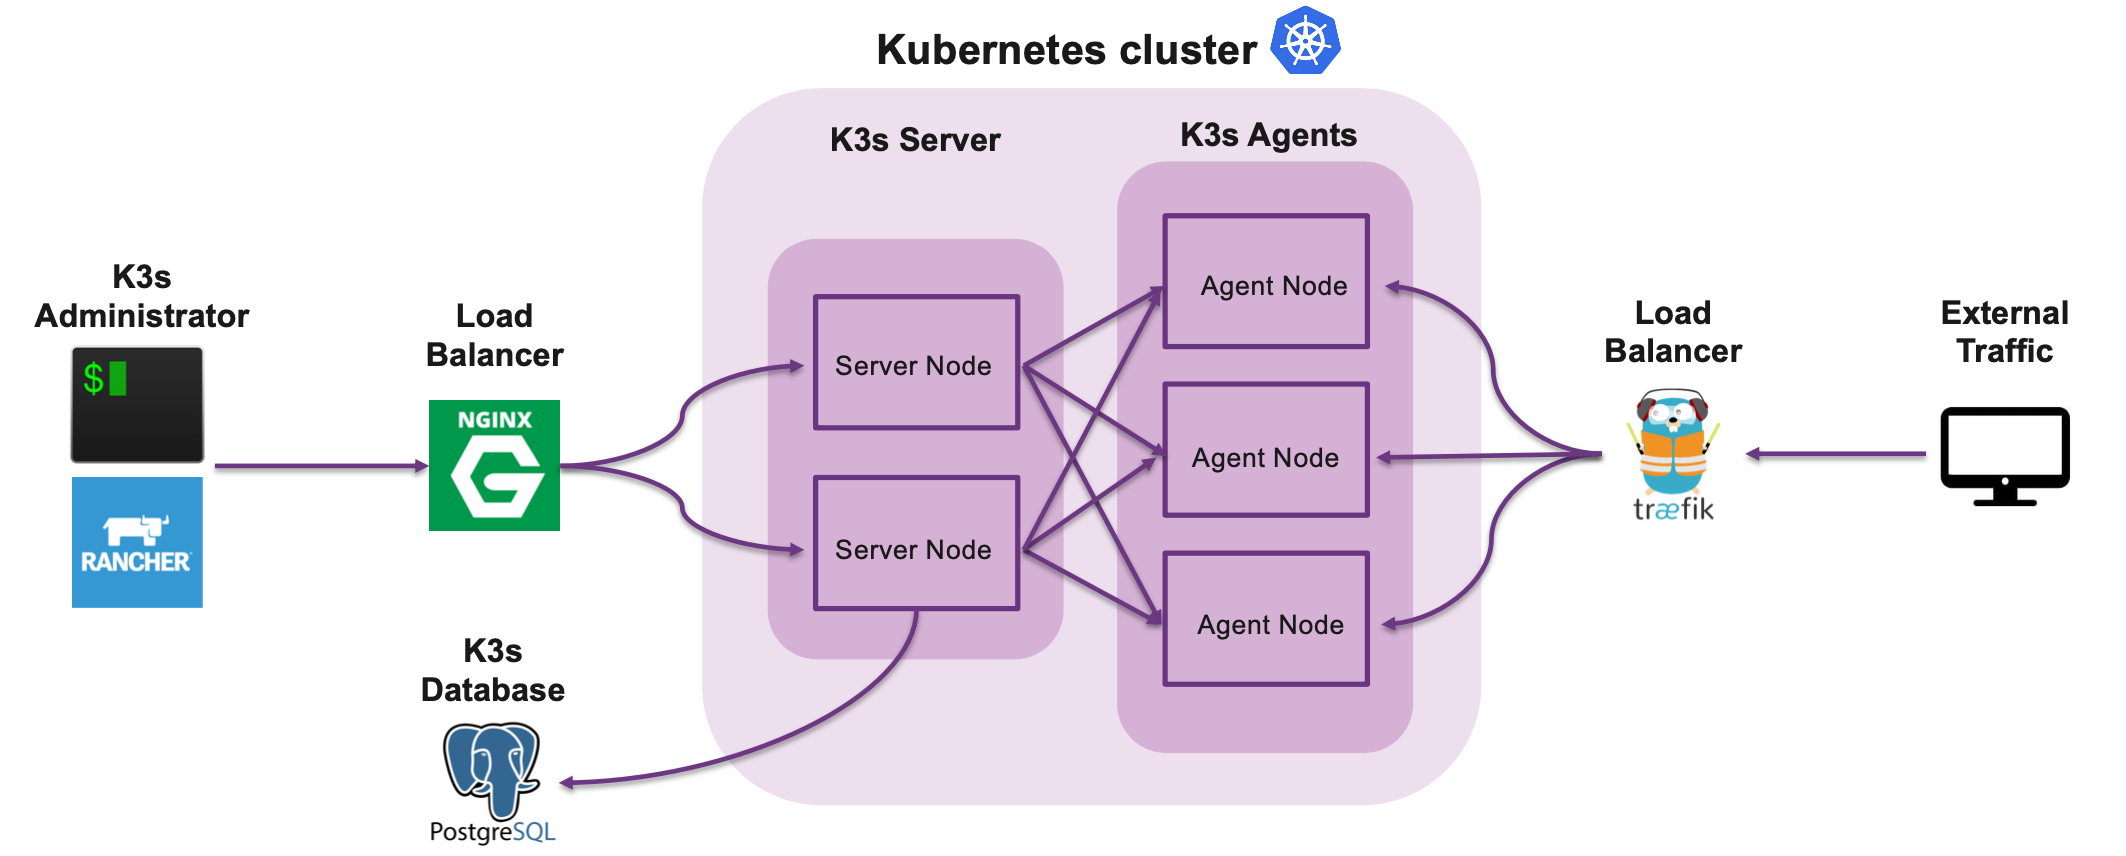
\includegraphics[width=\linewidth]{09-Deployment/kubernetes-architecture.png}
    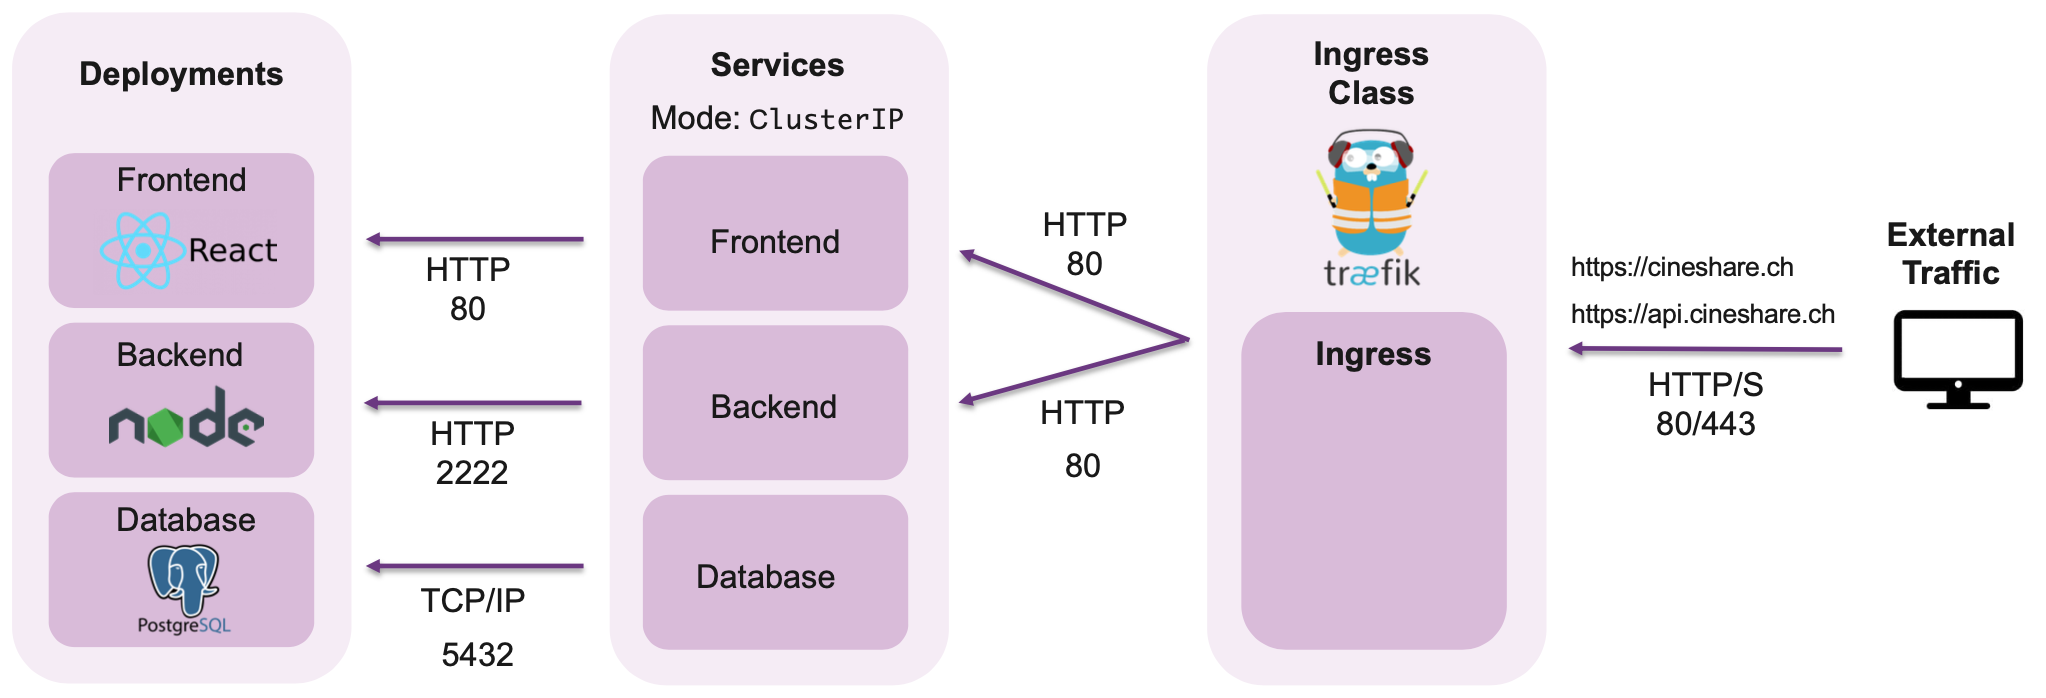
\includegraphics[width=\linewidth]{09-Deployment/kubernetes-arch2.png}
\end{center}
\vspace{-8pt}

\subsubsection{Units}
\begin{minipage}{.4\linewidth}
    \begin{itemize}
        \item Pod
        \item Service
        \item Deployment
        \item Ingress
        \item Namespace
        \item StatefulSet
        \item DaemonSet
    \end{itemize}    
\end{minipage}
\begin{minipage}{0.5\linewidth}
    \begin{center}
        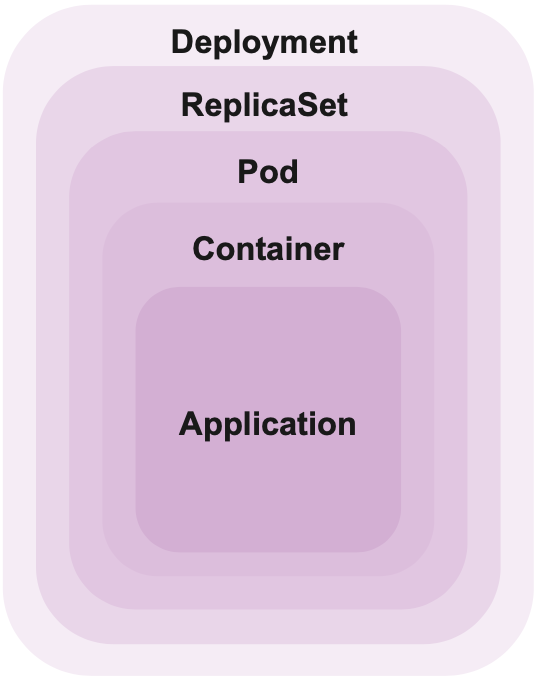
\includegraphics[scale=.3]{09-Deployment/kubernetes-units.png}
    \end{center}    
\end{minipage}

%\vspace{-8pt}

\subsection{Docker Swarm}
\subsubsection{Properties}
\begin{itemize}
    \item Deploy with docker-compose.yml
    \item swarm manager / swarm nodes architecture
    \item Built into docker
    \item Scheduler is responsible for placement of containers to nodes 
\end{itemize}

\subsubsection{Units}
\begin{center}
    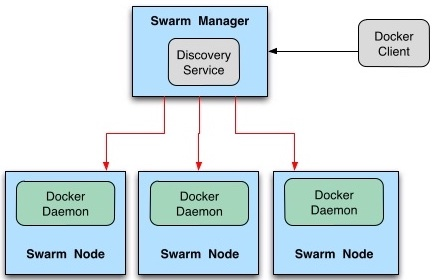
\includegraphics[scale=.25]{09-Deployment/docker-swarm.jpeg}
\end{center}
\vspace{-8pt}

\subsection{Summary}
\begin{itemize}
    \item Docker Swarm has already lost the battle against Kubernetes for supremacy in the container orchestration space
    \item Kubernetes supports higher demands with more complexity
    \item Docker Swarm offers a simple solution, quick to get started with
\end{itemize}